\chapter{Сёла Выгуровщина и Троещина}

Вскоре мы плотно займемся странным земляным сооружением – погребальным валом, отождествленным учеными с... остатками замка  князя Симеона Олельковича, а впридачу с летописным Городком. С этим я поспорю много дальше, тут бы сначала прояснить вопрос – а где было это, как говорит наука, «городище»?

Источники сообщают про известный в узком кругу вал на берегу озера Гнилуши. Поскольку оно неразрывно связана с селами Выгуровщиной и Троещиной, я расскажу сначала о них, и потом только двинемся дальше.

Современный жилмассив Вигуровщина-Троещина поглотил б\'ольшую часть села Выгуровщины, и лежит на восток от уцелевшего села Троещины. Мне придется постоянно уточнять, когда говорю о жилмассиве, а когда о селе. От села Выгуровщины по 2016 год осталась юго-западная часть.

Жили-были почти рядом два села. Троещина с некоторых времен до 1877 года, когда случилось большое наводнение, лежала севернее Выгуровщины, на берегу русла, что именуют теперь Десенкой. Потом Троещина переехала восточнее. По Выгуровщине серпом проходил также пруд, на карте лоций 1914 года подписанный как «оз. Ставок (б. пр.)», на карте Сноевского – «река Прудок», на карте 1719 года – «речка Пруд». 

Троещина названа потому, что это было владение Больницкого Троицкого Монастыря Киево-Печерской Лавры. Само село Троетчина известно с 18 века. Было к северу от нее и Троецкое озеро. А Выгуровщиной владел Ян Выгура, вроде бы завещавший село Михайловскому Златоверхому монастырю. Прежде на месте Выгуровщины находилось летописное селение Милославское. Кстати, была еще Милославщина у Витичевского брода, много южнее Киева.

С течением лет граница между Троещиной и Выгуровщиной менялась. По числу дворов Выгуровщина всегда преобладала. В 1766 году в Троещине было 28 дворов и 256 человек населения, а Выгуровщина в то же время насчитывала 42 двора с 409 душами. По состоянию на 1917 год, Троещина – 260 дворов, 1531 житель. Выгуровщина – 391 двор, 2210 душ. На 1939 год, Троещина – 436 дворов, 2099 жителей. Выгуровщина – 609 дворов, 2607 жителей.

К половине двадцатого века обжитые земли сёл соединились, однако формально объединение произошло в 1957 году – оба села записали в Троещину. Жители продолжали их различать, хотя не всегда правильно.

Различали еще и Оболонье, между Воскресенской слободкой и Выгуровщиной. Оболонье лежало у нынешнего перекрестка Ватутина и Бальзака, эдак от улицы Петра Вершигоры и включая первые номера домов на Бальзака. Официально, Оболонье было частью Выгуровщины, но местные издавна знали, что к чему. На стыке Оболонья и Троещины стоял сельмаг. Ходило два автобуса – номер 6 от Дарницы до Троещины и 25-й – со станции метро «Левобережная».

А восточнее, но также между Воскресенской Слободкой и Выгуровщиной, было болото Корчовня – его видно на немецкой карте 1943 года.

В 1981 году, после подвода трассы от Московского моста, село Троещину включили в состав Киева, и ту часть села, что была Выгуровщиной, начали сносить и на ее месте строить жилой массив Вигуровщина-Троещина, он же впоследствии просто Троещина.

Пространство бывшей Выгуровщины примерно обозначим как местность между улицами Кибальчича и Сабурова, словом – старая половина жилмассива Троещины. Село Троещина уцелело. От сельской Выгуровщины также остался кусочек, примыкающий с юга к селу Троещине. Кладбища у обоих сёл поныне разные! Выгуровское кладбище – между улицей Бальзака и Довженко\footnote{50°30'24"N 30°34'48"E}. Троещинское кладбище – между Пушкина и Садовой\footnote{\textasciitilde{}50°31'10"N 30°35'10"E}.

В частном секторе, всё по улице Карла Маркса и примыкающим к ней Довженко, Димитрова, Маяковского – это Выгуровщина. А всё, что вдоль другой основной дороги, улицы Ленина (ныне Радосыньской) – село Троещина. 

На Выгуровщине дома плоше, сохранилось больше старых. Уцелевший ныне кусочек Выгуровщины, в 1970-х и 90-х некоторыми жителями «восточной» Выгуровщины считался Троещиной. На всё село Троещину теперь только одна школа – №278, а было две, по одной на посёлок.

Немцы почти разрушили оба села во время Великой Отечественной. Жители Выгуровщины в 1941 году создали нехилый партизанский отряд из 170 человек, во главе которого встали Г. Н. Кузьменко и А. М. Светличный. Отряд был поделен на 4 боевые группы. К концу сентября того же года на их счету было 60 убитых гитлеровцев, 2 подбитые самоходки, 9 машин врага. Удалось с боем вызволить и 900 советских военнопленных граждан, под Борисполем и Дарницей. Но фронт отступил далеко, к Полтаве, и выгуровским партизанам самим неоткуда было ждать помощи.

В любой местности мой краеведческий взгляд выискивает самое запутанное дело, поэтому расскажу о церквях в Троещине и Выгуровщине, однако не буду говорить об экономике этих сел в прошлом, а экономика в 19-20 веках была такая – упор на скотоводство, ибо земля здесь стала родить худо и земледелие отодвинулось на второй план. Был у жителей Выгуровщины и свой промысел – плетение предметов из лозы. В начале 20 века кустари Выгуровщины поставляли на продажу в Киев, в сезон, до тридцати тысяч корзин, сундуков и детских колясок. Лозоплетением занимались и троещинцы.

В селе Троещино, в 19 веке была церковь святой Троицы. О ней ничего мне неизвестно кроме что в 1876 году она относилась к Вигуровщино-Слободскому приходу Черниговской губернии. К тому же приходу, но в Выгуровщине, относилась церковь святого Георгия. Несколько церквей на приход возможны, когда настоятель каждого храма – один и тот же священник.

Во второй половине 19 века, священник Николай Алексеевич Переяславец (Переяславцев) служил в Выгуровщине. Из казацкой семьи, он был человеком музыкальным, умел играть на скрипке, и в местечке Носовке создал церковный хор. То же организовал он и в Выгуровщине. 

Внук Николая Алексеевича, Федор Спасский в очерке «Памяти нескольких регентов и их певчих киевского района перед войной и во время нея» рассказал, что однажды дед его возвращался от черниговского епарха на пароходе. Около устья Десны сделали остановку на ночь. Переяславец услышал, как на берегу молодежь здорово поет. Утром пошел в село и встретился там со старым, больным священником. Тот искал себе замену, но из-за бедности прихода никто сюда не хотел. 

Переяславец вместе с этим священником составил прошение к архиепископу о переводе его, Николая Алексеевича, в Выгуровщину, а музыкально одаренной местной молодежи пообещал научить их петь по нотам, в церковном хоре. Прошение приняли, Переяславец перебрался в Выгуровщину и устроил тут хор, в репертуар коего вошли и светские песни. Чтобы его послушать, приезжали нарочно из Киева. Потомки Николая Алексеевича пошли по его стопам, становясь регентами церковных хоров.

Деревянную выгуровскую церковь святого Георгия построили еще в 1708 году, о чем сообщает очерк «Остёр и его уезд» в нумере 15 «Черниговских епархиальных известий» за 1863 год. Уже в 1766 году при церкви этой существовала школа, где жил дьяк, обучавший детей.

Дальнейшую судьбу этой церкви я выяснил только из письма Леонида Соболева, опубликованного в газете.

Леонид Аркадьевич Соболев родился в 1917 году. Из дворян. Жили на Трехсвятительской улице, около Андреевской церкви. Мать Леонида звали Евдокией, работала учительницей музыки в шестой школе. Отец же его был учителем рисования.

Соболев окончил музыкальную школу, и играл до старости на разных клавишных, включая синтезатор. Прошел курсы радистов, увлекался парашютизмом.

Великая Отечественная война застала его студентом последнего курса Киевского гидромелиоративного института. На фронт пошел добровольцем. Оборона Киева, 1 августа 1941 года. Около Жулян. Лезут танки, лейтенант Соболев из состава отдельного саперного батальона, подбивает один танк, и со связкой гранат бросается под другой. Подрывает его вместе с собой. Ранен в позвоночник и голову.

Раскрошило так, что знакомые много лет считали его погибшим. Прошел такой слух, о смерти. На войне погиб и отец Леонида, Аркадий, да младший брат Владимир.

Откопали Соболева из песка, привезли в военный госпиталь №408. Ко времени, когда Соболева выписали, Киев заняли немцы. Несколько подлечившийся Соболев ушел в религию, в 1942 году принял сан диакона. В 1945 году стал вегетарианцем. 

Много позже, в конце 20 века, при созданном им ските на Выгуровщине, Соболев устроил приют для бездомных собак и кошек. Жило там в вольерах чуть не по сотне и тех, и других. Сам Соболев, в то время – седой уже схиархимандрит Серафим – ходил со свитой из дворняжек. Учил своих прихожан с добром относиться к животным и брать к себе оных бездомных. Каких-то собак Соболев подбирал сам, других ему просто подкидывали. Потом они ходили к нему на могилу.

Помнили. Помнят и такое – при ските кормили не только собак, но и нищих. Инвалид первой группы, пенсию свою Соболев раздавал, кому нужно было. Красил себе волосы и бороду в ярко-красный цвет, носил обувь на босу ногу.

В 1947 году, окончив семинарию, Соболев получил приход в Бортничах. Тамошнюю церковь сожгли гитлеровцы, и Соболев начал сбор средств среди прихожан на новую. Строительство и отделка деревянного (сейчас его обложили кирпичом) храма Покрова Пресвятой Богородицы продолжались 13 лет. До сих пор стоит. Кисти Соболева принадлежат 50 икон в нем. В начале шестидесятых Соболева перевели служить в Троещину.

%На время прерву рассказ о нем и поведаю про две фотографии, найденные мною в сети. Где же еще?

В начале 21 века было уже неизвестно, как выглядели церкви в Троещине и Выгуровщине – Троицкая и Георгиевская. И вот в сети появились два снимка, один подписан как «Георгиевская церков с.Вигуровщина снимок 1940 года», другой «св.Троицкая церковь с. Троещина снимок»\footnote{В 2015 году выложили еще несколько фотографий, и назвали всё ту же церковь Георгиевской. Однако для меня вопрос остается нерешенным.}. Их обнаружили висящими на стене старого, заброшенного дома на Татарке. Чей дом, кто делал фотографии – неведомо.

%Начинается история, как обычно бывает с Киевом. Возникает множество действительностей одновременно, причем одна противоречит другой. Противоречивы между собой даже сами фотографии.

Фотография без даты, с подписью «св. Троицкая церковь с.Троещина снимок»:

\begin{center}
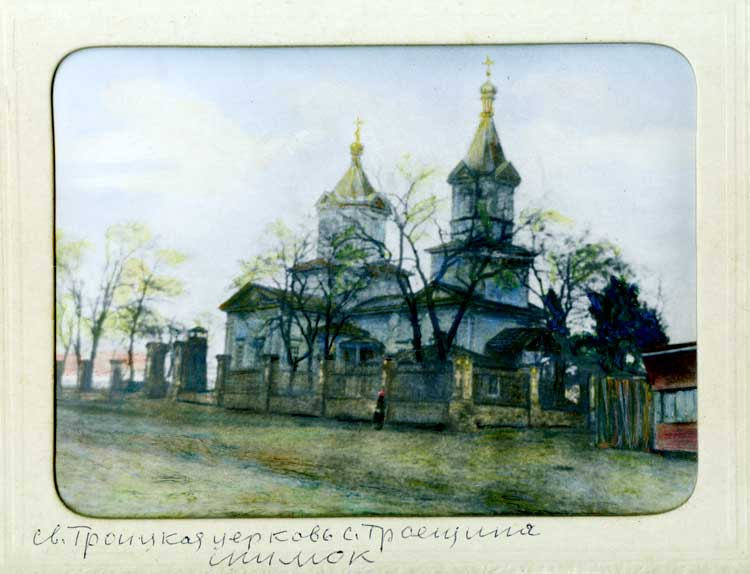
\includegraphics[width=0.93\linewidth]{chast-gorodki/vyg-troya/cerk-troick.jpg}
\end{center}

А вот фотография с подписью: «св. Георгиевская церков с. Выгуровщина снимок 1940 года». Да, мы знаем, что именно Георгиевская, деревянная церковь была на Выгуровщине испокон веков. Очевидно, что церковь запечатлена одна и та же. Но какая? И не ошибся ли человек, подписавший снимки?
\vspace*{\fill}
\begin{center}
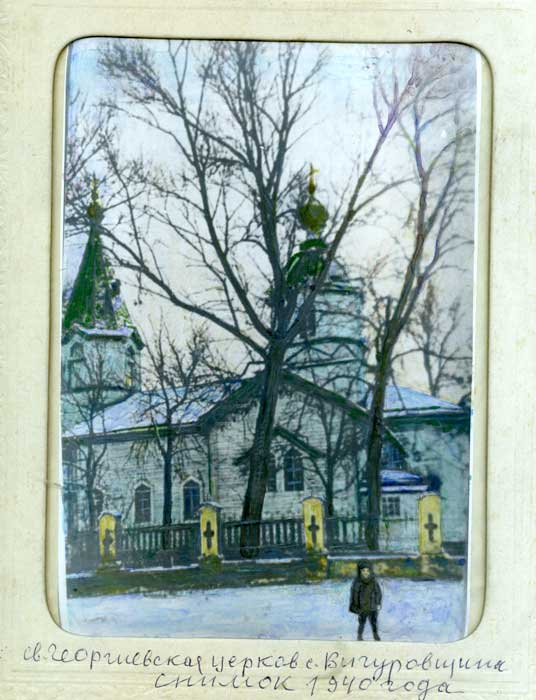
\includegraphics[width=\linewidth]{chast-gorodki/vyg-troya/cerk-georg.jpg}
\end{center}
\vspace*{\fill}
\newpage

В 1962 году на месте Троицкой церкви решили построить сельский клуб (это на 2014-й улица Ленина, 27)\footnote{В двухэтажом доме культуры с тремя залами вплоть до 21 века не было туалета и горячей воды. На 2014 год там работало несколько детских кружков – гитарный, хоровой, шахматный. Шахматы вел ветеран Давид Заид 1928 года рождения.}. Точнее, сначала запретили звонить в колокола, а затем постановили – церковь убрать, клуб поставить. За неделю до сноса предупредили. 

Священником храма был Соболев. Под его руководством прихожане объединенного уже села Троещины (Выгуровщина плюс Троещина) разобрали по досочке деревянную церковь и перенесли в тачках и на плечах на новое место, выбитое Соболевым под храм. Старожилы говорят о месте как о пустыре в двух километрах от села. Поросший лозой и бурьяном, частью заболоченный пустырь. Всем миром собрали церковь заново, управились в три недели.

Потом там в 1991–1997 годах возвели Свято-Троицкий каменный собор, его адрес на 2014 год – улица Кирова, 2-Б. Соболев тоже немало вложился в строительство, продав свою квартиру в центре на Трехсвятительской. А деревянную старую церковь приспособили под храм основанного Соболевым тут же Святодуховского скита (Свято-Духовский мужской скит Киево-Печерской лавры) – он прячется за собором, если глядеть со стороны трассы. Но прежнего полноразмерного деревянного храма больше не видно. 

Поныне для меня загадка, какая церковь изображена на двух фотографиях. Старожилы помнят Троицкую как «маленькую деревянную». Деревянной была и Георгиевская.

В 2005 году полковник в отставке, военный сослуживец Соболева, Антон Скульбашевский, среди бумаг покойного отыскал письмо, которое Соболев хотел отправить тогдашнему мэру Омельченко. В письме, относящегося ко времени, когда уже был построен скит при «малом Свято-Троицком храме», содержалась просьба о помощи в восстановлении церкви и колокольни Георгия Змееборца, сожженных фашистами в 1943-м.

Где же стояла она? 

Георгиевская церковь отмечена, по карте Шуберта 1863 года, на западном берегу Прудка, причем рядом, на другом берегу, была водяная мельница. Но план Шуберта именно от Выгуровщины с Троещиной и на север становится неточным, и я не знаю, как именно, посему не могу наложить его на современную эту местность. На более точных плане лоций 1914 года и РККА 1930-х, Прудок – серпообразный, и его полукруг точнехонько вписывается в современные улицы Бальзака (нумера 14-26) и улицу Каштановую. 

%Простодушное наложение карты на современную дает место церкви около дома 15-А по проспекту Маяковского (не улице Маяковского в Выгуровщине), примыкая к этому дому с востока. Но план Шуберта именно от Выгуровщины и Троещины становится неточным, и я не знаю, в какой мере и откуда именно. И Прудок, по нему, течет через Выгуровщину иначе, чем на последующих картах. Например на плане лоций 1914 года и РККА 1930-х, Прудок – серпообразный, и его полукруг точнехонько вписывается в современные улицы Бальзака (нумера 14-26) и улицу Каштановую. 

Да, о жители сих славных улиц – здесь еще не столь давно протекал Прудок, через него был мост (на месте дома по Каштановой 9), а примерно между школой №275 (Маяковского, 3-Г) и остановкой «Жилмассив Радужный» на проспекте Генерала Ватутина Прудок сливался с руслом, имя коего нам надлежит еще выяснить.

\begin{center}
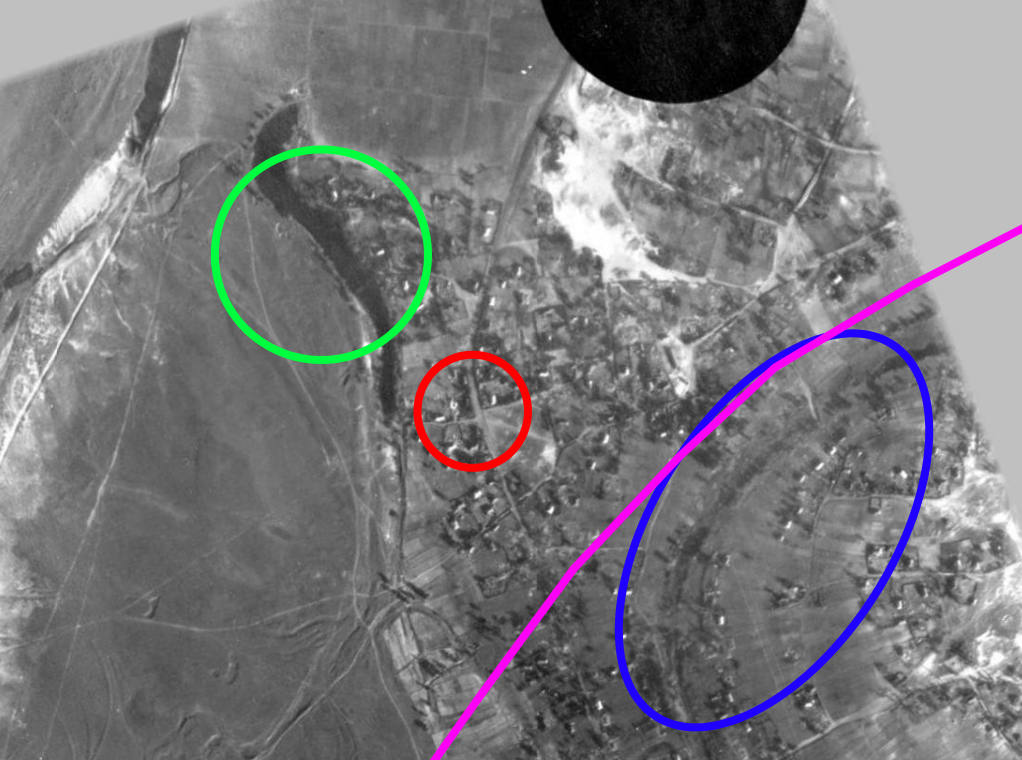
\includegraphics[width=\linewidth]{chast-gorodki/vyg-troya/troya-prudok.jpg}
\end{center}

На аэрофотоснимке 1943 года красным я отметил нынешний перекресток улиц Карла Маркса и Довженко, в синий овал вписывается полукруг Прудка, малиновая линия – линия скоростного трамвая вдоль современной улицы Бальзака, и салатовый кружок – озеро Гнилуша. К западу от него видно еще одно, подобное, по виду старица.

Что же случилось с Прудком? Старожилы вспоминают, что при застройке Выгуровщины высотками, речку загнали в «бетонные короба», и сверху стали намывать песок.

Остальные два водоема по 2023 год сохранились.
